\subsection{Fenugreek}
\label{sec:fenugreek}

\begin{spice}\label{spice:fenugreek}
\textsc{Fenugreek} \hfill \href{https://powo.science.kew.org/taxon/523957-1}{POWO} \\
\textbf{English:} \textit{fenugreek}. 
\textbf{Arabic:} {\arabicfont{حلبة}} \textit{ḥulba}. 
\textbf{Chinese:} {\tradchinesefont{胡蘆巴}} \textit{húlúbā}. 
\textbf{Hungarian:} \textit{görögszéna} [greek-hay].  \\
\noindent{\color{black}\rule[0.5ex]{\linewidth}{.5pt}}
\begin{tabular}{@{}p{0.25\linewidth}@{}p{0.75\linewidth}@{}}
Plant species: & \taxonn{Trigonella foenum-graecum}{L.} \\
Family: & \textit{Fabaceae/Leguminosae} \\
Plant part used: & seed; leaf \\
Region of origin: & S. Europe; W. Asia \\
Cultivated in: & India \\
Color: & mustard yellow seeds \\
\end{tabular}
\end{spice}

\begin{figure}[!ht]
	\vspace{-4ex}
	\centering
	\subfloat[\centering a]{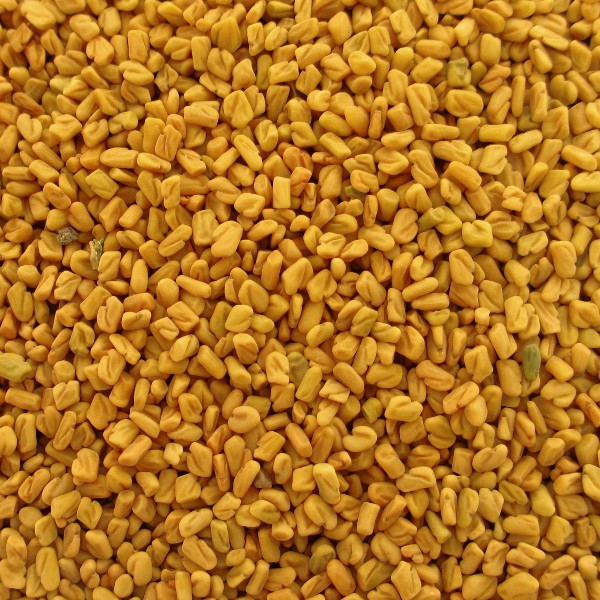
\includegraphics[width=0.3\linewidth]{imgs/spices/fenugreek-1.jpg}}
	\hfill
	\subfloat[\centering b]{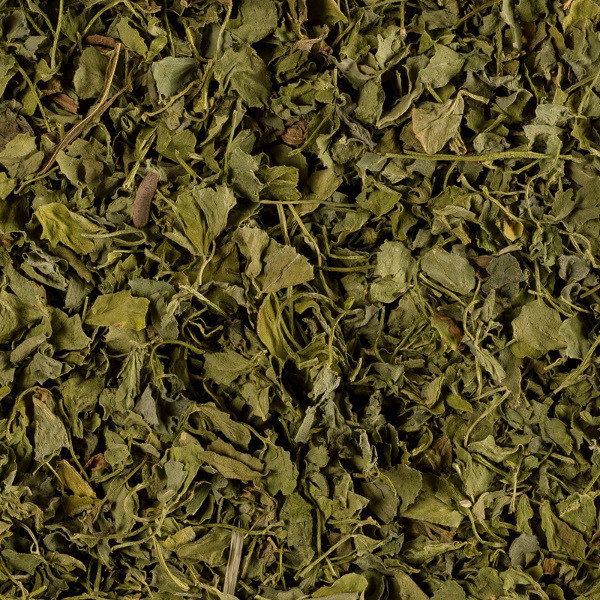
\includegraphics[width=0.3\linewidth]{imgs/spices/fenugreek-2.jpg}}
	% \hfill
	% \subfloat[\centering c]{\includegraphics[width=0.3\linewidth]{imgs/spices/fenugreek-3.jpg}}
	\caption{Fenugreek \taxon{}.}
	\label{fig:fenugreek_imgs}
\end{figure}

\subsection{The Botany of Fenugreek}

\subsection{The History of Fenugreek}

\subsection{The Names of Fenugreek}

\subsubsection{English}

\begin{etymology}\label{ety:fenugreek}
\textbf{English} \textit{fenugreek}, in old English from Latin, in Middle English and later from French
< \textbf{French} \textit{fenugrec}
< \textbf{Latin} \textit{faenugraecum} [Greek-hay], named \textit{faenum Graecum} `Greek hay' by the Romans\footnote{}
\end{etymology}

\begin{table}[!ht]
    \caption{Various names for fenugreek in English.}
\centering
\begin{tabularx}{\textwidth}{@{}l>{\itshape \small}lL>{\small}l@{}}
\toprule
\textbf{\#} & \multicolumn{1}{l}{\textbf{Species}} & \multicolumn{1}{l}{\textbf{Name}} & \multicolumn{1}{l}{\textbf{Source}} \\
\midrule
\textbf{1}	& \textbf{Trigonella foenum-graecum}	& \textbf{fenugreek}	& \textbf{\textcite{van_wyk_culinary_2014}} \\
2	& Trigonella foenum-graecum	& fenugreek-seed	& \textcite{oed} \\
\bottomrule
\end{tabularx}
\label{table:names_fenugreek_en}
\end{table}



\subsubsection{Arabic}

\begin{table}[!ht]
    \caption{Various names for fenugreek in Arabic.}
\centering
\begin{tabularx}{\textwidth}{@{}l>{\itshape \small}lr>{\itshape}lL>{\small}l@{}}
\toprule
\textbf{\#} & \multicolumn{1}{l}{\textbf{Species}} & \multicolumn{1}{l}{\textbf{Name}} & \multicolumn{1}{l}{\textbf{Tr.}} & \multicolumn{1}{l}{\textbf{Gloss}} & \multicolumn{1}{l}{\textbf{Source}} \\
\midrule
\textbf{1}	& \textbf{Trigonella foenum-graecum}	& \textbf{حلبة}	& \textbf{ḥulba}	& \textbf{}	& \textbf{\textcite{lane_arabic-english_1863}} \\
\bottomrule
\end{tabularx}
\label{table:names_fenugreek_ar}
\end{table}



\subsubsection{Chinese}

\begin{table}[!ht]
\centering
\begin{tabularx}{\textwidth}{@{}l>{\itshape \small}ll>{\itshape}lL>{\small}l@{}}
\toprule
\textbf{\#} & \multicolumn{1}{l}{\textbf{Species}} & \multicolumn{1}{l}{\textbf{Name}} & \multicolumn{1}{l}{\textbf{Tr.}} & \multicolumn{1}{l}{\textbf{Gloss}} & \multicolumn{1}{l}{\textbf{Source}} \\
\midrule
\textbf{1}	& \textbf{Trigonella foenum-graecum}	& \textbf{\tradchinesefont{胡蘆巴}}	& \textbf{húlúbā}	& \textbf{phonetic}	& \textbf{\textcite{kleeman_oxford_2010}} \\
\bottomrule
\end{tabularx}
\caption{Various names for fenugreek in Chinese.}
\label{table:names_fenugreek_zh}
\end{table}



\subsubsection{Summary}

\begin{table}[!ht]
    \caption{Conventionalized names for fenugreek in English, Arabic, and Chinese, found in dictionaries.}
\centering
\begin{tabularx}{\textwidth}{@{}ll>{\itshape}lLl>{\small}l@{}}
\toprule
\textbf{\#} & \textbf{Language} & \multicolumn{1}{l}{\textbf{Term}} & \textbf{Gloss} & \textbf{Loan} & \multicolumn{1}{l}{\textbf{Source}} \\
\midrule
1	& English	& fenugreek	& 	& yes	& \textcite{oed} \\
2	& English	& fenugreek-seed	& 	& no	& \textcite{oed} \\
\midrule
\midrule
1	& Chinese	& húlúbā	& barbarian-reeds-ba	& yes	& \textcite{kleeman_oxford_2010} \\
\bottomrule
\end{tabularx}
\label{table:names_fenugreek}
\end{table}





% check Wehr for aabic expl